%Allahu Akbar

Berbagai penelitian dilakukan untuk mengembangkan sistem deteksi pada robot sejak lama. Proyek \textit{capstone} ini membangun sebuah sistem deteksi manusia dan benda khusus  untuk robot \covid. Robot COVID-19 yang dimaksud pada dokumen ini adalah robot yang dapat bergerak secara otomatis membantu tugas-tugas tenaga kesehatan dan meminimalkan interaksi langsung dari tenaga kesehatan dengan pasien. Sistem ini bertujuan untuk menambah kemampuan robot COVID-19 agar memiliki kemampuan untuk membedakan manusia dengan objek benda mati lainnya yang nantinya berperan menjadi dasar untuk pengembangan fungsi-fungsi lebih lanjut robot dalam membantu tenaga kesehatan.
%Semangat BSD Season 4 mau tayang uhuy


\section{Robot \textit{Autonomous}}
\label{sec:Robot_Autonomous}

    Robot adalah produk dari bidang robotika di mana mesin dapat diprogram dan dibangun untuk membantu manusia atau meniru tindakan manusia. Robot pada awalnya dibangun untuk menangani tugas-tugas monoton (seperti membuat mobil di jalur perakitan pabrik), tetapi semakin lama robot semakin berkembang jauh hingga dapat melakukan tugas-tugas seperti memadamkan api, membersihkan rumah, dan membantu operasi yang sangat rumit. Setiap robot memiliki tingkat otonomi yang berbeda mulai dari robot yang dikendalikan manusia yang melakukan tugas yang dikendalikan sepenuhnya oleh manusia hingga robot yang sepenuhnya \auto\ yang melakukan tugas tanpa perintah eksternal.
    
    Robot \auto\ merupakan robot yang mampu memutuskan aksinya untuk mengeksekusi perintah secara mandiri tanpa campur tangan manusia hingga tujuan tercapai\cite{b1}. Robot ini memanfaatkan berbagai sensor untuk memperoleh informasi dan menggunakan hasil pelatihan data untuk memutuskan apa yang akan dilakukan. Robot dapat diklasifikasikan sebagai robot \auto\ jika mereka kemampuan dalam persepsi, pengambilan keputusan dan aktuasi secara mandiri. Walaupun robot ini tidak memerlukan tenaga manusia saat beroperasi, robot ini masih memerlukan manusia untuk melakukan perawatan secara berkala.

    Robot \auto\ saat ini dioperasikan dalam berbagai bidang dalam kehidupan sehari-hari. 
    Robot \auto\ biasa digunakan dalam transportasi logistik misal dalam \textit{e-commerce} menggunakan robot \auto\ untuk melakukan transportasi barang, pemenuhan pesanan, penyortiran, dan pengatur penyimpanan. Robot ini juga digunakan untuk mengangkat barang berat dan mengangkut barang ke seluruh ruangan dalam gudang-gudang. 
    Robot \auto\ dalam industri umumnya memiliki bagian tambahan khusus seperti lengan dan konveyor untuk memudahkan produksi dan distribusi.
    % This also enables instant, accurate, and easily accessible documentation of the process.
    
    \begin{figure}[!ht]
        \centering
        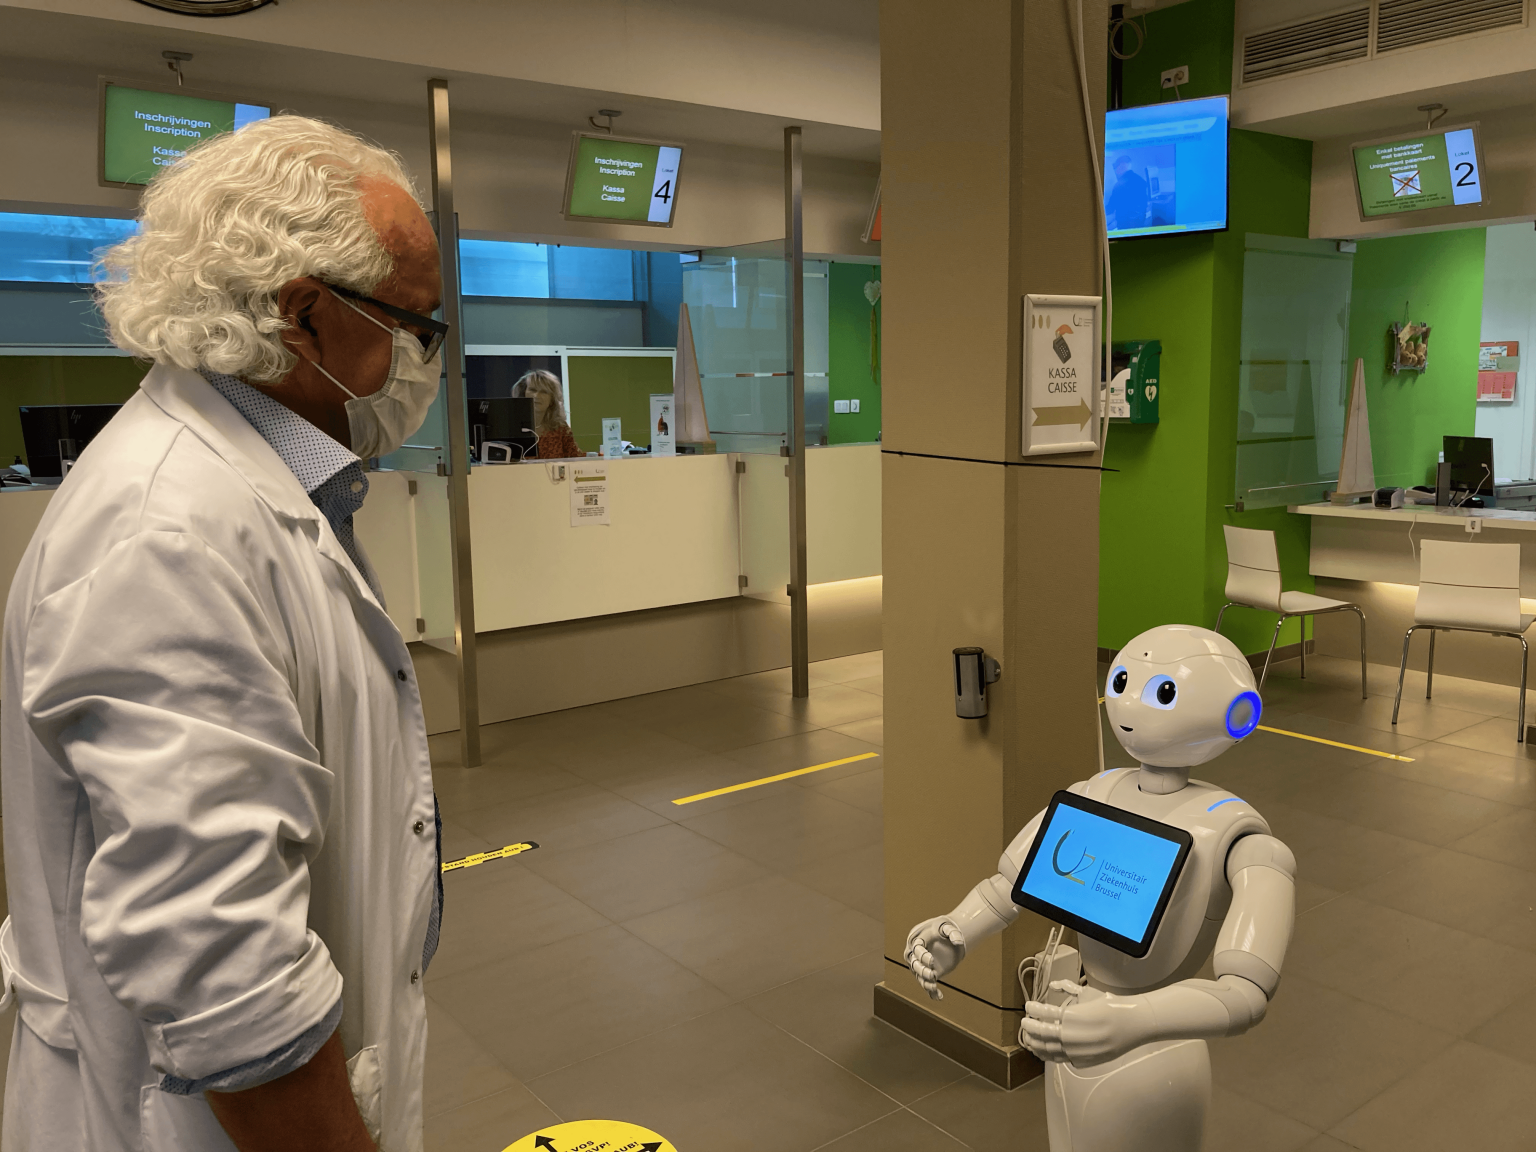
\includegraphics[scale=0.3]{robot_cruzr.png}
        \caption{Robot \textit{Autonomous} CRUZR di Rumah Sakit Belgium\cite{b2.1}.}
        \label{fig:Ch02_robot_CRUZR}
    \end{figure}
    
    Saat ini robot \auto\ juga mulai dikembangkan dalam bidang kesehatan karena dapat memberikan berbagai keuntungan seperti aman, andal, dan mampu untuk memproduksi obat secara efisien\cite{b2}. Gambar \ref{fig:Ch02_robot_CRUZR} merupakan salah satu robot bidang kesehatan yang telah dikembangkan adalah robot CRUZR yang bekerja di \textit{Antwerp University Hospital} di Belgium\cite{b2.1}. Robot ini mempunyai tugas untuk menyapa pasien, mengecek suhu tubuh dan masker pasien, kemudian mengantar pasien ke ruang yang ingin dituju. Robot ini beroperasi secara mandiri tanpa operator manusia. Hal ini memberikan kelebihan yaitu berkurangnya kontak antara tenaga kesehatan dengan pasien pada masa pandemi \covid\ ini.
    
%   contoh robot??
   
   
\section{Sensor Kamera dan Sensor Jarak}
\label{sec:sensor}  
   Ada berbagai sensor yang dapat digunakan robot untuk membaca dan memetakan lingkungan sekitar tanpa memerlukan kontak fisik. Sensor-sensor ini dapat bekerja untuk menentukan jarak objek di sekitarnya hingga dapat memberi gambaran bentuk objek target. 
   
   \subsection{Sensor Kamera}
    \label{subsec:Sub-Metode_Kamera}
    
    Robot \auto\ memiliki kemampuan seperti \textit{Obstacle Avoidance (OA), Augmented Reality (AR), Simultaneous Localization and Mapping (SLAM),} dan \textit{Mobile Object Tracking (MOT)} yang semuanya membutuhkan informasi akurat mengenai posisi objek di lingkungan. Pendeteksian objek menggunakan kamera yang biasanya dapat mengetahui jarak target untuk memperoleh informasi lengkap seperti letak dan tekstur target. Kamera yang memiliki kemampuan tersebut disebut dengan kamera RGB-D (\textit{Red, Green, and Blue - Depth}). Kamera RGB-D memberikan informasi berupa gabungan visual warna, bentuk dan kedalaman untuk mengenali target\cite{b3}. Contoh hasil bacaan kamera RGB-D diperlihatkan pada Gambar \ref{fig:Ch02_rgbd_kamera}.
    \begin{figure}[!ht]
        \centering
        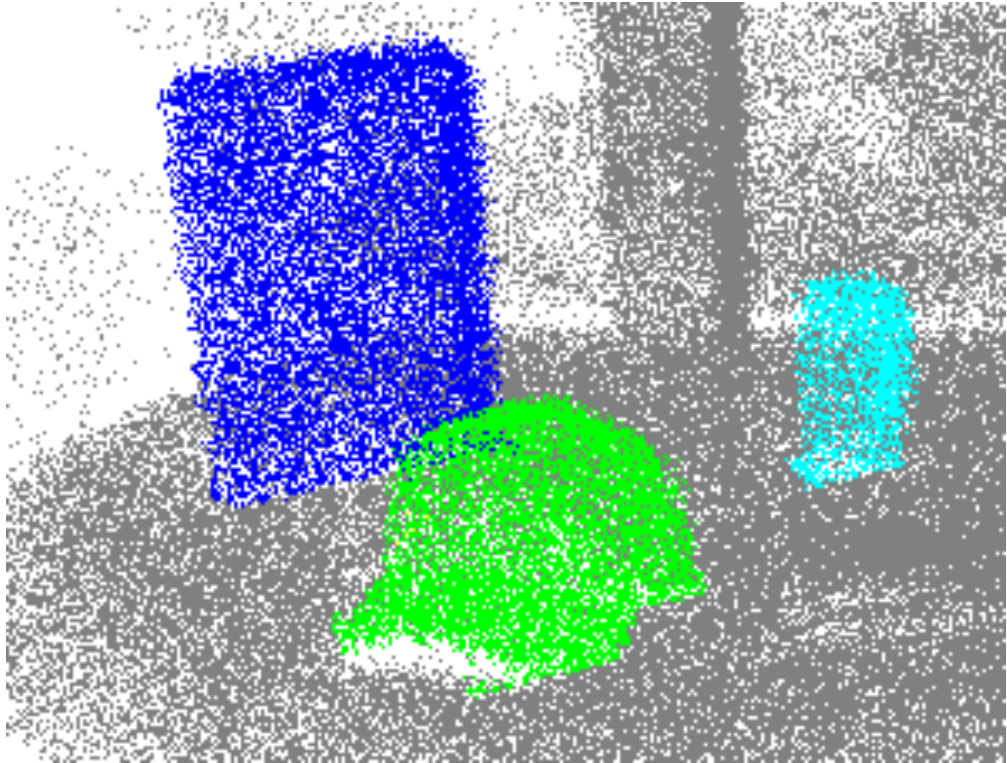
\includegraphics[scale=0.3]{rgbd.png}
        \caption{Contoh hasil bacaan kamera RGB-D\cite{b3}.}
        \label{fig:Ch02_rgbd_kamera}
    \end{figure}
    
    \subsection{Sensor Jarak}
    \label{subsec:Sub-Metode_Laser}
    
    Sensor jarak menentukan jarak target dengan memancarkan suatu sinyal kemudian menunggu kembalinya sinyal tersebut. Sensor-sensor ini banyak digunakan untuk robot, mobil, \textit{drone}, dan berbagai teknologi lainnya yang memerlukan kemampuan pengukuran jarak.
    
        \subsubsection{Sensor Ultrasonik}
        \label{subsec:Ultrasonik}
        Sensor ini memancarkan gelombang ultrasonik untuk mengukur jarak dengan target. Sensor akan menghitung waktu antara pancaran dengan pantulan untuk menghitung jarak. Sinyal ultrasonik memiliki kisaran frekuensi 30 kHz hingga 5 MHz yang dapat digunakan untuk menghasilkan pulsa. Frekuensi tinggi memiliki panjang gelombang yang lebih rendah sehingga resolusi akan menjadi lebih baik, tetapi semakin tinggi frekuensi dapat menghasilkan atenuasi yang juga semakin tinggi. Sensor dengan frekuensi rendah memiliki keuntungan tingkat hamburan rendah dan lebih murah, tetapi panjang gelombangnya di udara hanya beberapa milimeter sehingga memerlukan perawatan khusus\cite{b4}.
        \begin{figure}[H]
            \centering
            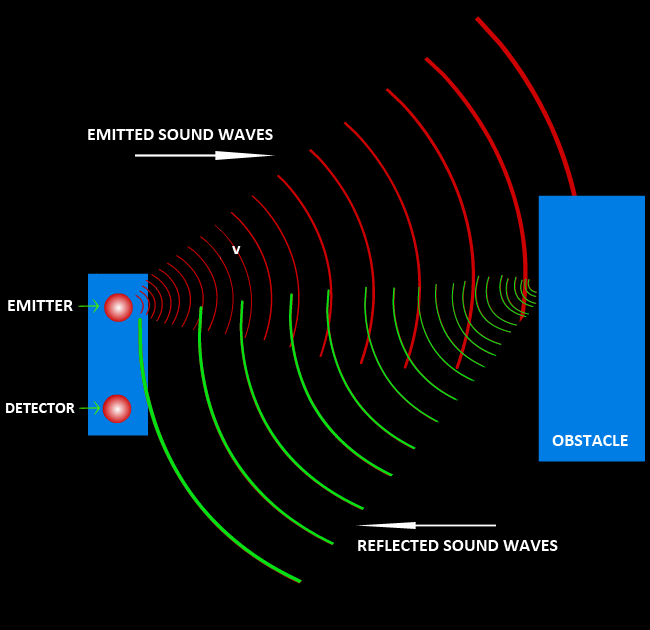
\includegraphics[scale=0.5]{CH02_Ultrasonic.png}
            \caption{Cara kerja sensor ultrasonik\cite{b_g1}.}
            \label{fig:Ch02_ultrasonik}
        \end{figure}
        Seperti yang terlihat pada Gambar \ref{fig:Ch02_ultrasonik}, \textit{emiter} pada sensor ini akan memancarkan gelombang dan \textit{detector} akan menangkap gelombang pantul. Gelombang suara ultrasonik yang dikeluarkan adalah getaran pada frekuensi di atas jangkauan pendengaran manusia (\>20kHz) yang dapat merambat melalui berbagai media (udara atau cairan).
        
        Untuk menghitung jarak antara sensor dan objek, sensor mengukur waktu yang diperlukan antara pengeluaran gelombang oleh pemancar hingga kontaknya dengan penerima. Rumus untuk perhitungan ini adalah \[D = \frac{1}{2}T * C\] 
        \newline \noindent dengan keterangan:
        \begin{itemize}
            \item D: jarak;
            \item T: waktu;
            \item C: kecepatan suara (343 meter/detik).
        \end{itemize}
        
        Sensor ultrasonik digunakan sebagai sensor jarak. Sensor ini dapat ditemukan dalam teknologi parkir mobil otomatis dan sistem keamanan anti-tabrakan. Sensor ultrasonik juga digunakan dalam sistem deteksi rintangan robot, serta teknologi manufaktur. Dibandingkan dengan sensor inframerah (IR) dalam aplikasi penginderaan jarak, sensor ultrasonik tidak rentan terhadap gangguan asap, gas, dan partikel udara lainnya (meskipun komponen fisik masih dipengaruhi oleh variabel seperti panas).
        
        \subsubsection{Sensor Inframerah}
        \label{subsec:Infrared}
        
        \begin{figure}[H]
            \centering
            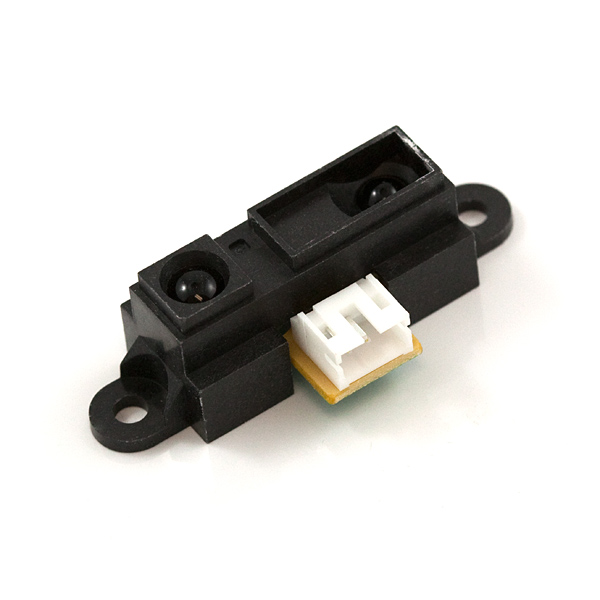
\includegraphics[scale=0.3]{infrared_sensor.jpg}
            \caption{Sensor Jarak Inframerah\cite{b_g2}.}
            \label{fig:Ch02_inframerah}
        \end{figure}
        
        Sensor inframerah (sensor IR) adalah komponen \textit{optoelectronic} yang sensitif terhadap radiasi dengan sensitivitas spektral dalam rentang panjang gelombang inframerah \SI{780}{\nano\metre} hingga \SI{50}{\micro\metre}\cite{b5}. 
        Sensor yang terlihat pada Ganbar \ref{fig:Ch02_inframerah} tersebut banyak digunakan sebagai detektor gerakan misalnya dalam gedung untuk menyalakan lampu atau dalam sistem alarm untuk mendeteksi penyusup. Sensor mendeteksi radiasi panas (radiasi inframerah) yang berubah seiring waktu dan ruang karena adanya pergerakan. Sensor ini juga banyak digunakan dalam perangkat peringatan gas, penganalisis gas, teknologi pengukuran gas medis, detektor api, dan pengukuran suhu presisi tanpa kontak. 

        Ada dua jenis sensor inframerah yaitu aktif dan pasif. Sensor inframerah aktif memancarkan dan mendeteksi radiasi inframerah. Sensor IR aktif memiliki dua bagian yaitu \textit{light-emitting diode} (LED) dan penerima. Ketika sebuah objek mendekati sensor, cahaya inframerah dari LED memantul dari objek dan dideteksi oleh penerima. Sensor IR aktif bertindak sebagai sensor jarak, dan biasanya digunakan dalam sistem deteksi rintangan (seperti pada robot). Sensor inframerah pasif (PIR) hanya mendeteksi radiasi inframerah dan tidak memancarkannya dari LED.

        \subsubsection{Sensor \lidar (\textit{Light Detection and Ranging})}
        \label{subsec:lidar_sensor}
        
        
         \lidar\ (juga disebut LADAR) merupakan sensor optik yang digunakan untuk mengukur jarak dengan cara menembakkan cahaya ke target kemudian menangkap pulsa cahaya tersebut untuk dihitung jaraknya.  \lidar\ menggunakan sinar ultraviolet, cahaya tampak, atau inframerah agar dapat mendeteksi berbagai jenis target termasuk benda non-logam, batuan, hujan, dan senyawa kimia lainnya. Sinar laser dapat digunakan untuk memetakan fitur fisik dengan resolusi yang sangat tinggi. Saat ini \lidar\ dimanfaatkan untuk berbagai keperluan seperti mengukur jarak, menghitung kecepatan target bergerak, membaca lingkungan, mengestimasi lokasi target dan lain sebagainya. 
         
         \lidar\ memiliki beberapa jenis antara lain yaitu \lidar\ 1D, \lidar\ 2D, dan \lidar\ 3D. Hal yang membedakan ketiganya adalah jumlah dimensi hasil bacaan. Pada Gambar \ref{fig:Ch02_3d_bacaan} terlihat hasil bacaan \lidar\ 3D yang memiliki 3 sumbu X,Y, dan Z.
         \begin{figure}[H]
            \centering
            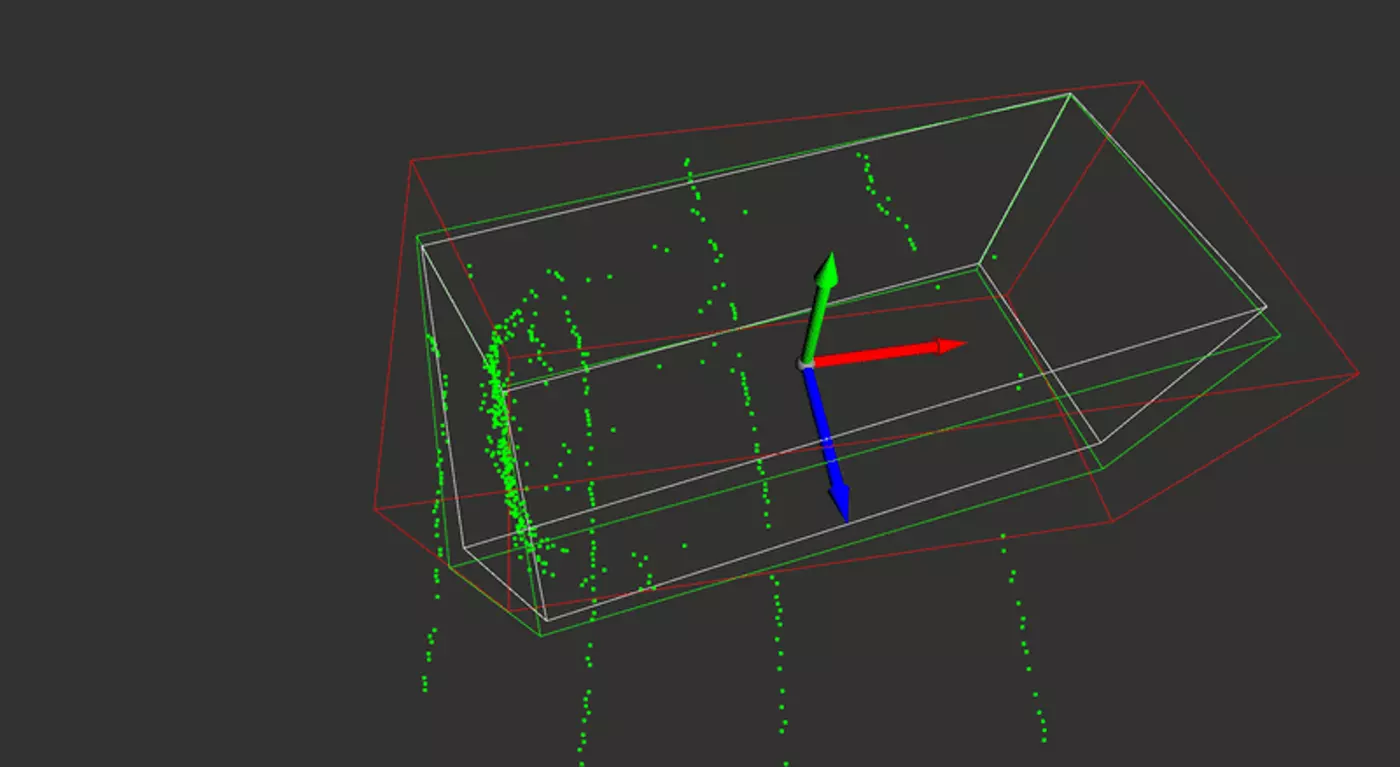
\includegraphics[scale=0.3]{3D_lidar_scanan.png}
            \caption{Contoh hasil bacaan \lidar\ 3D\cite{b_g2}.}
            % https://understand.ai/blog/annotation/machine-learning/autonomous-driving/2021/03/29/3D-vs-2D-sensor-data-for-machine-perception.html
            \label{fig:Ch02_3d_bacaan}
        \end{figure}
    
         \lidar\ memiliki keunggulan jarak jangkauan lebih tinggi, resolusi tinggi, dan kecepatan memindai yang lebih tinggi dari sensor-sensor jarak yang disebutkan sebelumnya. Tidak seperti kamera, \lidar\ berfungsi secara independen dari pencahayaan sekitar sehingga dapat memperoleh hasil yang baik saat siang dan malam tanpa kehilangan performa akibat gangguan seperti bayangan, sinar matahari, atau silau cahaya lampu \cite{b6}. Oleh karena itu, proyek ini akan menggunakan \lidar\ sebagai sensor utama untuk mendapatkan gambaran objek sekitar.

% Robot Operating System
\section{Sistem Operasi Robot}
\label{sec:ROS} 

    Berbagai sistem operasi untuk robot saat ini telah dikembangkan. Sistem-sistem ini dapat digunakan untuk memprogram dan mensimulasikan robot dengan lebih mudah.
    Sebelum ada pengembangan sistem operasi robot, setiap \dev\ membuat program dari awal yang biasanya tidak bisa langsung diaplikasikan dan dikembangkan ke dalam robot lain.
    Berbagai sistem operasi dan program muncul untuk menjadi platform umum pada pengembangan aplikasi robotika. Berbagai sistem dapat digunakan untuk tujuan komersial maupun penelitian secara gratis dan \textit{open source}. Adanya algoritma siap pakai yang sudah tersedia dan dukungan komunitas yang besar membuat pengembangannya lebih mudah.
    
    \textit{Robot Operating System} (ROS) merupakan salah satu perangkat lunak khusus pengembangan robot yang bersifat \textit{open source} dengan \textit{libraries} dan \textit{tools} yang sudah tersedia untuk membangun program pada robot. ROS memiliki fitur yang banyak. Biasanya \dev\ menggunakan ROS untuk membuat prototipe, ROS tidak digunakan untuk membuat produk sebenarnya dikarenakan berbagai alasan seperti keamanan dan kekurangan pada pemrosesan \textit{real-time}\cite{b7}. Proyek \textit{capstone} ini menggunakan ROS karena sistem ini sudah digunakan untuk mengembangkan robot \covid\ yang telah ada.
    \noindent Beberapa fitur ROS yang mendukung pengembangan robot antara lain yaitu:
    \begin{itemize}
     \item ROS menyediakan antarmuka penyampaian pesan untuk komunikasi antara dua program atau proses.
     \item ROS bukanlah sistem operasi yang sebenarnya tetapi merupakan sistem operasi meta yang menyediakan beberapa fungsi dan fitur mirip sistem operasi asli.
     \item Mendukung bahasa pemrograman tingkat tinggi dan berbagai \textit{tools}.
     \item Kerangka kerja ROS terintegrasi dengan berbagai \textit{libraries} yang populer seperti OpenCV dan PCL.
     \item algoritma siap pakai.
     \item ROS mudah digunakan untuk pembuatan prototipe.
     \item Dukungan komunitas.
     \item \textit{Tools} dan simulator yang luas.
     \end{itemize}
% Why use ros?
% This is common question that developers ask when looking for a platform to program ROS. Although ROS has many features, there are still areas in which ROS can’t be used or is not recommended to use. In the case of a self-driving car, for example, we can use ROS to make a prototype, but developers do not recommend ROS to make the actual product. This is due to various issues, such as security, real-time processing, and so forth. ROS may not be a good fit in some areas, but in other areas, ROS is an absolute fit. In corporate robotics research centers and at universities, ROS is an ideal choice for prototyping. And ROS is used in some robotics products after lot of fine-tuning (but not self-driving cars).
% There was active development in robotics before the ROS project, but there was no common platform and community for developing robotics applications. Each developer created software for their own robot, which in most cases, couldn’t be reused for any other robot. Developers had to rewrite code from scratch for each robot, which takes a lot of time. Also, 
% most of the code was not actively maintained, so there was no support for 
% the software. Also, developers needed to implement standard algorithms 
% on their own, which took more time to prototype the robot.
% After the ROS project, things changed. Now there is a common platform for developing robotics applications. It is free and open source for commercial and research purposes. Off-the-shelf algorithms are readily available, so there is no longer a need to code. There is big community support, which makes development easier. In short, the ROS project changed the face of robotics programming.

\section{\textit{Object Recognition}}
\label{sec:object_detection} 

\textit{Object recognition} adalah bentuk aplikasi dasar untuk pemrosesan gambar dan \textit{vision} pada komputer. Istilah ini digunakan dalam berbagai aplikasi dan algoritma. Secara umum \objd\ bertujuan untuk mengingat data tentang penampilan objek tertentu dan memeriksa untuk mengevaluasi objek tersebut jenis apa dan di mana letaknya. 

\begin{figure}[H]
            \centering
            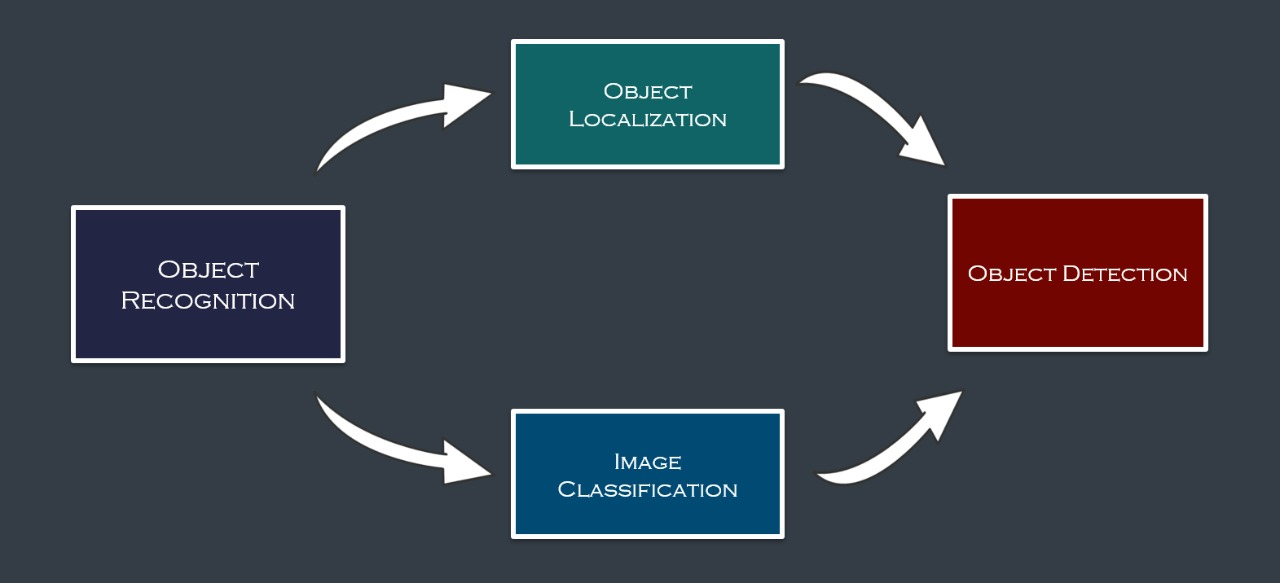
\includegraphics[scale=0.3]{Object_Rec.jpeg}
            \caption{Diagram Proses \textit{Object Recognition}.}
            \label{fig:Ch02_objectR}
        \end{figure}

Pada Gambar \ref{fig:Ch02_objectR} terlihat bahwa dalam object recognition terdapat dua proses terpisah yaitu \textit{object localization} dan \textit{image classification}. \textit{object localization} merupakan komponen untuk menentukan posisi dan jarak benda atau objek yang terdeteksi disekitar lingkungan. Image classification berfungsi untuk mengklasifikasi jenis objek yang terdeteksi. Kedua proses ini kemudian digabungkan menjadi \textit{object detection}. \textit{Object detection} biasanya menampilkan hasil klasifikasi dan letak objek hasil pemrosesan dalam \textit{bounding box} dengan keterangan nama objek. 

Ada banyak pendekatan yang berbeda untuk merancang \objd\, masing-masing memperhitungkan tuntutan spesifik dari konteks aplikasi yang diinginkan. Kategorisasi metode dan mode operasi dapat dikelompokkan melalui beberapa kriteria yang mengacu pada properti model data yang mewakili objek dan mode operasi skema \objd. Kriteria-kriteria tersebut adalah sebagai berikut\cite{b8}:
\begin{itemize}
\item Representasi objek: Terdapat dua cara informasi tentang objek dapat diidentifikasi yaitu dengan geometri atau penampilan. Informasi geometris mengacu pada batas atau  bentuk permukaan objek. Sementar itu, model berbasis tampilan diturunkan dari karakteristik potret wilayah yang dicakup oleh objek.
\item Cakupan data objek: Data model dapat merujuk pada properti lokal objek (contoh: posisi sudut objek) atau karakteristik objek global (contoh: area, keliling, momen inersia).
\item Variasi objek yang diharapkan: Kriteria lain adalah varians yang dapat ditunjukkan oleh individu yang berbeda dari kelas objek yang sama.
\item Kualitas data gambar: Kualitas data juga memiliki dampak signifikan pada desain algoritma.
\item Strategi pencocokan: Untuk mengenali objek dalam gambar memerlukan langkah pencocokan di beberapa titik dalam aliran algoritma misalnya pada model objek harus disejajarkan dengan konten gambar dengan cara kesamaan antara model dan gambar dimaksimalkan atau perbedaan diminimalkan.
\end{itemize}

%Sumber dari buku An Introduction to Object Recognition